\documentclass{article}
% LOL no sé como usarlo... empezamos bien.
\usepackage{tikz}
% Configuring tikz 
\usetikzlibrary{arrows,shapes.geometric,positioning,matrix,calc}
\tikzset{
  invisible/.style={inner sep=0pt}
  ishikawa/.style={align=center, inner sep=0pt},
  matter/.style  ={rectangle, minimum size=10mm, very thick, draw=red!70!black!40,
    top color=white, bottom color=red!50!black!20, font=\itshape, font=\scriptsize},
  level_1/.style ={ellipse, node distance=6pt, minimum size=6mm, very thick,
    draw=red!50!black!50, top color=white, bottom color=red!50!black!20, font=\itshape, font=\scriptsize},
  level_2/.style={rectangle, minimum size=6mm, font=\itshape, font=\tiny}}
\tikzset{
  rows/.style 2 args={@/.style={row ##1/.style={#2}},@/.list={#1}},
  cols/.style 2 args={@/.style={column ##1/.style={#2}},@/.list={#1}},
}
\begin{document}
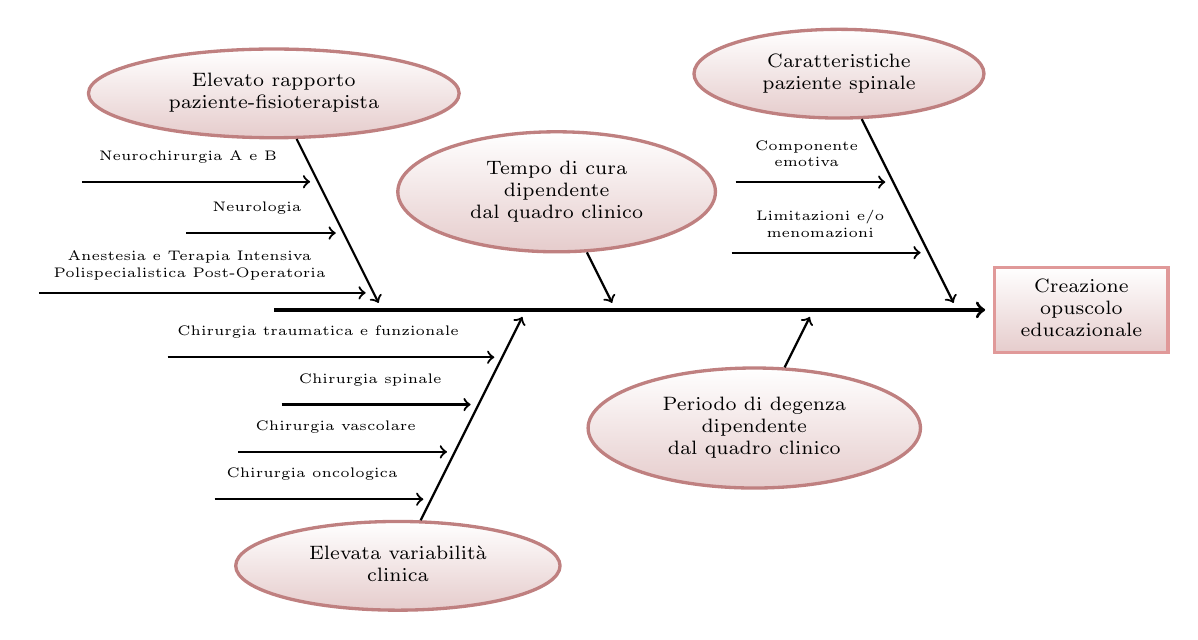
\begin{tikzpicture}

\tikzset{
toarr/.style={->, shorten <=+0pt, shorten >=+.1cm, thick},
toarr1/.style={->, shorten <=+0pt, shorten >=+.1cm, very thick}
}


\node[matter](effetto){
    \begin{tabular}{c}
        Creazione\\opuscolo\\ educazionale
    \end{tabular}
};

\draw[toarr1] ($(effetto) + (-10.25,0)$) -- (effetto) 
node[invisible, pos= 0.15](I1) {}
node[invisible, pos= 0.35](I2) {}
node[invisible, pos= 0.475](I3) {}
node[invisible, pos= 0.75](I4) {}
node[invisible, pos= 0.95](I5) {};

%CAUSA 1
\node[matter, level_1, 
yshift=2.75cm, xshift=-1.375cm, 
node distance = 3cm
](causa1) at (I1) {
    \begin{tabular}{c}
        Elevato rapporto\\paziente-fisioterapista
    \end{tabular}
};

\draw[toarr] (causa1) -- (I1.center)
node[pos=0.25,invisible] (SC11) {}
node[pos=0.55,invisible] (SC12) {}
node[pos=0.9, invisible] (SC13) {}
;

\draw[toarr] ($(SC11) + (-3,0)$) -- (SC11.center) 
node[invisible, pos= 0.45,
above, level_2] {Neurochirurgia A e B};

\draw[toarr] ($(SC12) + (-2,0)$) -- (SC12.center) 
node[invisible, pos= 0.45,
above, level_2] {Neurologia};

\draw[toarr] ($(SC13) + (-4.25,0)$) -- (SC13.center) 
node[invisible, pos= 0.45,
above, level_2] {\begin{tabular}{c}
Anestesia e Terapia
Intensiva\\Polispecialistica Post-Operatoria
\end{tabular}};

%CAUSA 2
\node[matter, level_1, 
yshift=-3.25cm, xshift=-1.625cm, 
node distance = 3cm
](causa2) at (I2) {
    \begin{tabular}{c}
        Elevata variabilità\\clinica
    \end{tabular}
};

\draw[toarr] (causa2) -- (I2.center)
node[pos=0.10,invisible] (SC21) {}
node[pos=0.325,invisible] (SC22) {}
node[pos=0.55, invisible] (SC23) {}
node[pos=0.775, invisible] (SC24) {}
;

\draw[toarr] ($(SC21) + (-2.75,0)$) -- (SC21.center) 
node[invisible, pos= 0.45,
above, level_2] {Chirurgia oncologica};

\draw[toarr] ($(SC22) + (-2.75,0)$) -- (SC22.center) 
node[invisible, pos= 0.45,
above, level_2] {Chirurgia vascolare};

\draw[toarr] ($(SC23) + (-2.5,0)$) -- (SC23.center) 
node[invisible, pos= 0.45,
above, level_2] {Chirurgia spinale};

\draw[toarr] ($(SC24) + (-4.25,0)$) -- (SC24.center) 
node[invisible, pos= 0.45,
above, level_2] {Chirurgia traumatica e funzionale};

%CAUSA 3
\node[matter, level_1, 
yshift=1.5cm, xshift=-.75cm, 
node distance = 3cm
](causa3) at (I3) {
    \begin{tabular}{c}
        Tempo di cura\\dipendente\\ dal quadro clinico
    \end{tabular}
};
    
\draw[toarr] (causa3) -- (I3.center);

%CAUSA 4
\node[matter, level_1, 
yshift=-1.5cm, xshift=-.75cm, 
node distance = 3cm
](causa4) at (I4) {
    \begin{tabular}{c}
        Periodo di degenza\\dipendente\\ dal quadro clinico
    \end{tabular}
};

\draw[toarr] (causa4) -- (I4.center);

%CAUSA 5
\node[matter, level_1, 
yshift=3cm, xshift=-1.5cm, 
node distance = 3cm
](causa5) at (I5) {
    \begin{tabular}{c}
        Caratteristiche\\paziente spinale
    \end{tabular}
};

\draw[toarr] (causa5) -- (I5.center)
node[pos=0.33,invisible] (SC51) {}
node[pos=0.7,invisible] (SC52) {}
;

\draw[toarr] ($(SC51) + (-2,0)$) -- (SC51.center) 
node[invisible, pos= 0.45,
above, level_2] { \begin{tabular}{c}
  Componente \\ emotiva
\end{tabular}};

\draw[toarr] ($(SC52) + (-2.5,0)$) -- (SC52.center) 
node[invisible, pos= 0.45,
above, level_2] {
\begin{tabular}{c}
Limitazioni e/o\\ menomazioni
\end{tabular}};
\end{tikzpicture}
\end{document}
